\documentclass[11pt]{article}

% --- Packages ---
\usepackage[margin=1in]{geometry}
\usepackage{mathptmx}
\usepackage[utf8]{inputenc}
\usepackage[T1]{fontenc}
\usepackage{amsmath,amssymb,amsfonts}
\usepackage{graphicx}
\usepackage{booktabs}
\usepackage{caption}
\usepackage{hyperref}
\usepackage{xcolor}
\usepackage{array}
\usepackage{enumitem}
\usepackage{natbib}
\usepackage{fancyhdr}

% --- Hyperlink setup ---
\hypersetup{
  colorlinks=true,
  linkcolor=blue,
  citecolor=blue,
  urlcolor=blue,
}

% --- Header ---
\pagestyle{fancy}
\fancyhf{}
\fancyhead[C]{\small \textit{Working Paper.} \texttt{doi:10.5281/zenodo.20470971}}
\fancyfoot[C]{\thepage}
\renewcommand{\headrulewidth}{0pt}

% --- Title ---
\title{\textbf{Fin-JEPA: Joint-Embedding Predictive Representation Learning\\for Financial Time Series}}

\author{\textbf{Yihan Wang}\thanks{First author. \texttt{wangyihan@gmail.com}} \\[4pt]
  \texttt{\url{https://github.com/cedricwyh/fin-jepa}} \\[4pt]
  \textbf{Team Fin-JEPA}}

\date{}

\begin{document}

\maketitle

% =============================================================================
% Abstract
% =============================================================================
\begin{abstract}
We present Fin-JEPA, the first application of the Joint-Embedding Predictive Architecture (JEPA) to financial time series. Fin-JEPA learns 64-dimensional latent representations of daily equity features through a lightweight 367K-parameter architecture comprising a PriceEncoder (MLP with GELU activations, LayerNorm) and a TransformerPredictor with 4-layer causal Transformer (\texttt{n\_heads=4}, \texttt{embed\_dim=64}). Representational collapse is prevented through Sketched Isotropic Gaussian Regularization (SIGReg, $\lambda=0.1$). On a large-scale dataset of 6,230 publicly traded equities spanning 2010--2026 (2.07M training samples), the training loss converges from 1.369 to 0.706 over 50 epochs with no collapse (\texttt{stdZ}=1.35, \texttt{eff\_rank}=37.8). The learned latent predictions outperform an identity baseline by 10.1\% (\texttt{Z\_pred} MSE 0.2922 vs.\ 0.3249), confirming that daily financial time series contain learnable temporal structure. In downstream evaluation, we analyze prediction error (VoE) as a potential trading signal across 300 stocks (393K windows), finding weak-to-negligible signal (AUC$\approx$0.49, Spearman $r\approx$0). We outline future work for PELT-based regime detection and multi-horizon training.
\end{abstract}

% =============================================================================
% 1. Introduction
% =============================================================================
\section{Introduction}

Self-supervised representation learning for financial time series has largely followed two paradigms. Contrastive methods~\citep{oord2018representation,chen2020simclr} learn representations by maximizing agreement between augmented views of the same data, but their reliance on handcrafted augmentations---often poorly suited to the low signal-to-noise ratio of financial data---limits their effectiveness. Generative or reconstructive approaches~\citep{kingma2014vae,hochreiter1997lstm} learn compressed representations through an encoder--decoder bottleneck, but the reconstruction objective dedicates representational capacity to modeling irreducible noise components that are inherently unpredictable in financial markets.

The Joint-Embedding Predictive Architecture (JEPA), proposed by~\citet{lecun2022path}, offers a third path: learn representations by predicting the latent encoding of a future or masked signal from a context signal, without ever decoding back to the input space. By operating entirely in latent space, JEPA avoids the need to reconstruct noisy low-level details and instead learns representations that capture only the information necessary for temporal prediction. JEPA has demonstrated strong empirical performance in computer vision~\citep{assran2023ijepa} and video~\citep{bardes2024vjepa}, and has recently been adapted to general time series~\citep{ennadir2025tsjepa}. However, no prior work applies JEPA specifically to financial time series, which present unique challenges: extreme non-stationarity, heteroscedastic volatility, and a signal-to-noise ratio among the lowest in any prediction domain.

In this work, we make the following contributions:

\begin{enumerate}[leftmargin=*,nosep]
  \item \textbf{First application of JEPA to financial time series.} We design and validate Fin-JEPA, a lightweight architecture (367K parameters) combining a PriceEncoder with GELU activations and a TransformerPredictor with causal masking, trained with SIGReg regularization to learn predictive latent representations from daily equity data.
  \item \textbf{Large-scale empirical validation.} We train on 2.07 million samples from 6,230 publicly traded equities (2010--2026) and demonstrate stable convergence with no representational collapse (eff\_rank=37.8, stdZ=1.35). The model's latent predictions outperform an identity baseline by 10.1\%.
  \item \textbf{Comprehensive architecture ablation.} We evaluate 15 architecture variants (varying latent dimension, encoder/predictor depth, predictor type, and encoder type) on the HS300 stock universe, establishing that a deep predictor (6-layer Transformer), moderate latent dimension ($D=64$), and MLP-based encoder yield the best validation loss (1.8595).
  \item \textbf{Downstream VoE analysis.} We analyze predictor error (Variance of Error) as a divergence-based trading signal, finding that JEPA prediction errors do not provide statistically significant forward return discrimination.
\end{enumerate}

% =============================================================================
% 2. Related Work
% =============================================================================
\section{Related Work}

\textbf{Self-supervised learning for time series.}
SSL methods for time series can be broadly categorized into generative, contrastive, and predictive approaches. Generative methods, including LSTM autoencoders~\citep{srivastava2015unsupervised} and variational autoencoders~\citep{kingma2014vae}, learn representations through reconstruction; they are simple to train but tend to capture noise-dominated features in financial data. Contrastive methods, such as TS2Vec~\citep{yue2022ts2vec} and TS-TCC~\citep{eldele2021tstcc}, maximize agreement between augmented views and achieve strong performance on time series classification benchmarks, but require careful augmentation design and can suffer from false negative issues. Predictive methods directly model temporal dynamics; JEPA belongs to this family but distinguishes itself by predicting in latent space rather than reconstructing the input.

\textbf{JEPA and its variants.}
The JEPA framework was formalized by~\citet{lecun2022path} as an alternative to both contrastive and generative SSL. I-JEPA~\citep{assran2023ijepa} applies JEPA to images by predicting the latent representations of masked image blocks from a context block, achieving strong ImageNet performance without handcrafted augmentations. V-JEPA~\citep{bardes2024vjepa} extends the approach to video, predicting spatiotemporally masked regions. Most recently, TS-JEPA~\citep{ennadir2025tsjepa} adapts JEPA to general time series data, validating on UCR/UEA classification benchmarks and demonstrating that JEPA matches or surpasses existing SSL methods on standard time series tasks. Our work differs from TS-JEPA in targeting the financial domain with its unique non-stationarity and low signal-to-noise ratio, and in using a Transformer predictor (rather than MLP) with GELU activations. Additionally, MTS-JEPA~\citep{he2026mtsjepa} explores multi-resolution JEPA for anomaly detection with a codebook bottleneck, a complementary direction that does not address financial time series.

\textbf{Representation learning for finance.}
Financial representation learning has been explored through various lenses: LSTM-based autoencoders for anomaly detection in limit order books~\citep{lin2021anomaly}, variational autoencoders for portfolio construction~\citep{chen2022vae}, and contrastive learning for cross-sectional stock representations~\citep{sawhney2021contrastive}. None of these works employ a JEPA-style latent prediction objective with a Transformer predictor.

\textbf{Change-point detection and regime identification.}
PELT~\citep{killick2012pelt} provides an exact, computationally efficient algorithm for change-point detection under a penalized likelihood framework. While PELT has been applied to financial time series directly on price or volatility features~\citep{ross2013pelt,truong2020cpdetect}, the use of learned latent representations as input to PELT remains an open direction that we flag for future work.

% =============================================================================
% 3. Method
% =============================================================================
\section{Method}

\subsection{Problem Formulation}

Let $\mathbf{x}_t \in \mathbb{R}^d$ denote the observed feature vector at trading day $t$, consisting of technical features derived from price and volume data (22 dimensions). Given a historical context window of length $T$, $\mathcal{X}_t = \{\mathbf{x}_{t-T+1}, \dots, \mathbf{x}_t\}$, the objective is to learn an encoder function $f_\theta: \mathbb{R}^d \to \mathbb{R}^k$ that maps each observation to a latent representation $\mathbf{z}_t = f_\theta(\mathbf{x}_t)$, and a predictor function $g_\phi$ that predicts future latents from the sequence of past context latents:

\begin{equation}
\hat{\mathbf{z}}_{t+\tau} = g_\phi(\mathbf{z}_{t-T+1}, \dots, \mathbf{z}_t),
\label{eq:prediction}
\end{equation}

where $\tau$ is the prediction horizon (in the full training, $\tau$ corresponds to predicting the next 10 time steps autoregressively from 30 context steps). The encoder and predictor are trained jointly such that the predicted latent $\hat{\mathbf{z}}_{t+\tau}$ matches the true latent $\mathbf{z}_{t+\tau} = f_\theta(\mathbf{x}_{t+\tau})$ in representation space, without ever decoding either back to the input space. This predictive objective in latent space, as opposed to the generative reconstruction of denoising autoencoders or the contrastive alignment of siamese networks, constitutes the defining characteristic of the JEPA family~\citep{lecun2022path}.

\subsection{Architecture}

The complete architecture is implemented as \textbf{Fin-JEPA}, consisting of a PriceEncoder, a TransformerPredictor, and a SIGReg regularizer. Figure~\ref{fig:architecture} provides an overview.

\begin{figure}[t]
  \centering
  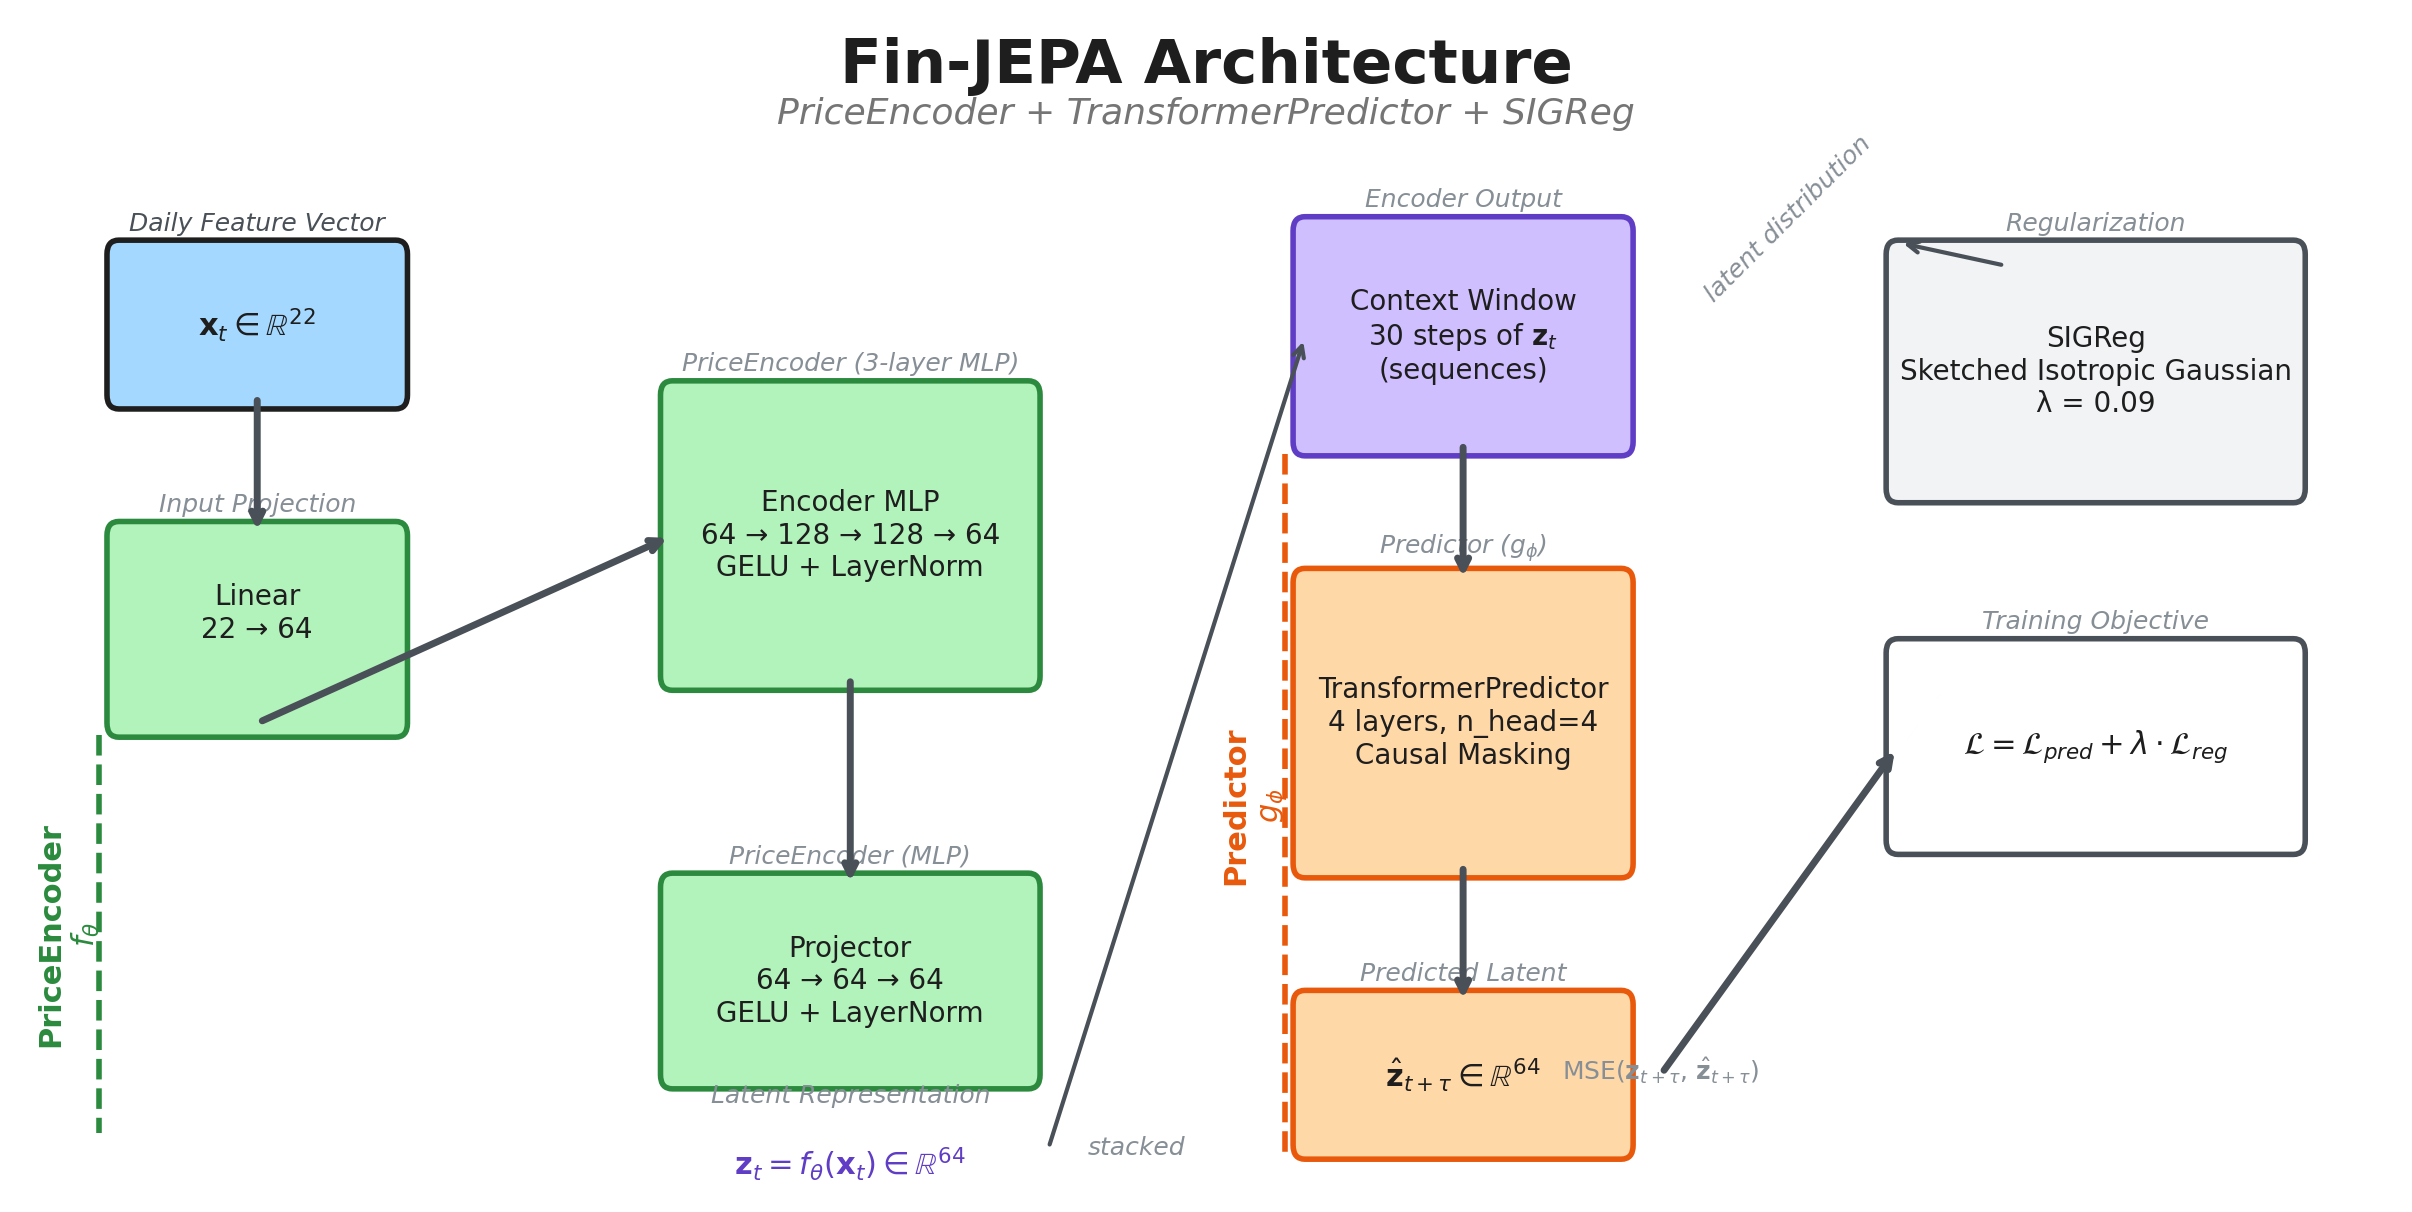
\includegraphics[width=0.85\textwidth]{figures/fig_architecture.png}
  \caption{\textbf{Fin-JEPA architecture overview.} The PriceEncoder maps each daily feature vector $\mathbf{x}_t$ to a latent $\mathbf{z}_t$. The TransformerPredictor operates causally in latent space, predicting $\hat{\mathbf{z}}_{t+\tau}$ from context latents. SIGReg regularizes the latent distribution to prevent collapse.}
  \label{fig:architecture}
\end{figure}

\textbf{Encoder (PriceEncoder).}
The encoder $f_\theta$ maps each daily feature vector $\mathbf{x}_t \in \mathbb{R}^{22}$ to a latent representation $\mathbf{z}_t \in \mathbb{R}^{64}$. It consists of three components:

\begin{itemize}[nosep]
  \item \textbf{Input projection:} $\texttt{nn.Linear}(22, 64)$ --- projects raw features to the embedding dimension.
  \item \textbf{Encoder MLP:} A 3-layer MLP with GELU activations and LayerNorm:
  \begin{equation}
  \texttt{LayerNorm} \to \texttt{Linear}(64\to 128) \to \texttt{GELU} \to \texttt{Linear}(128\to 128) \to \texttt{GELU} \to \texttt{Linear}(128\to 64)
  \end{equation}
  \item \textbf{Projector:} A 2-layer MLP with GELU and LayerNorm:
  \begin{equation}
  \texttt{LayerNorm} \to \texttt{Linear}(64\to 64) \to \texttt{GELU} \to \texttt{Linear}(64\to 64)
  \end{equation}
\end{itemize}

All hidden activations use \textbf{GELU}~\citep{hendrycks2016gelu}. No batch normalization or dropout is used; LayerNorm provides training stability while preserving the deterministic feedforward structure essential for latent-space prediction.

\textbf{Predictor (TransformerPredictor).}
The predictor $g_\phi$ operates entirely in latent space and is a causal Transformer encoder:

\begin{itemize}[nosep]
  \item \textbf{Position embedding:} Learned positional encodings of shape $(1, \texttt{max\_seq\_len}=256, 64)$.
  \item \textbf{Transformer blocks:} 4 layers of $\texttt{nn.TransformerEncoderLayer}$ with:
    $d_{model}=64$, $n_{head}=4$, $dim_{feedforward}=256$, $\texttt{activation}=\texttt{'gelu'}$, $\texttt{batch\_first}=\texttt{True}$, $\texttt{norm\_first}=\texttt{True}$, $\texttt{dropout}=0.1$.
  \item \textbf{Causal masking:} Upper triangular mask ($-\infty$ above diagonal) ensures each position can only attend to past and current positions.
  \item \textbf{Output projection:} $\texttt{LayerNorm} \to \texttt{Linear}(64\to 64) \to \texttt{GELU} \to \texttt{Linear}(64\to 64)$
\end{itemize}

The Transformer predictor is a critical design choice: unlike the MLP predictors used in I-JEPA/TS-JEPA, the causal attention mechanism enables the model to learn temporal dependencies across the context window, which is essential for financial time series where sequential structure matters.

\textbf{SIGReg --- Sketched Isotropic Gaussian Regularization.}
To prevent representational collapse, we apply SIGReg~\citep{balestriero2025lejepa}, which projects latent vectors onto random directions and matches their distribution to a standard Gaussian. The regularization randomly projects the $D$-dimensional latents onto 128 random directions using a normalized random matrix, then computes a kernel-based statistic comparing the empirical characteristic function to that of $\mathcal{N}(0,1)$. The SIGReg loss is added to the prediction loss with weight $\lambda = 0.1$.

\textbf{Parameter count.}
With $d=22$, $k=64$, 4-layer Transformer predictor (4 heads), and 3-layer encoder MLP, the total parameter count is approximately 367K for the best variant (v4\_deep\_d64). The model is lightweight enough for single-GPU training and real-time inference on a per-stock basis.

\subsection{Training Objective}

The training loss comprises two terms: a prediction loss $\mathcal{L}_{\text{pred}}$ that measures latent-space alignment, and a regularization loss $\mathcal{L}_{\text{reg}}$ that prevents representational collapse.

\textbf{Prediction loss.}
We define the prediction loss as the mean squared error (MSE) between the predicted and true latent representations:

\begin{equation}
\mathcal{L}_{\text{pred}} = \mathbb{E}_{t} \left[ \left\| \hat{\mathbf{z}}_{t+\tau} - \mathbf{z}_{t+\tau} \right\|_2^2 \right],
\label{eq:pred_loss}
\end{equation}

where the expectation is taken over time steps $t$ in the training set.

\textbf{Distribution regularization (SIGReg).}
To prevent the latent representations from collapsing to a low-dimensional subspace, we adopt Sketched Isotropic Gaussian Regularization. The regularization term encourages the empirical distribution of latents $\{\mathbf{z}_t\}$ to match a standard Gaussian prior $\mathcal{N}(0, I_k)$:

\begin{equation}
\mathcal{L}_{\text{reg}} = \text{SIGReg}(\{\mathbf{z}_t\}, \mathcal{N}(0, I_k)),
\label{eq:reg_loss}
\end{equation}

which is computed by projecting latents onto random directions and matching the empirical characteristic function to that of a standard Gaussian~\citep{balestriero2025lejepa}. The number of random projections is set to 128.

\textbf{Total objective.}
The combined loss is:

\begin{equation}
\mathcal{L} = \mathcal{L}_{\text{pred}} + \lambda \cdot \mathcal{L}_{\text{reg}},
\label{eq:total_loss}
\end{equation}

with $\lambda = 0.1$. This weighting ensures that prediction fidelity dominates the optimization while the regularization term provides a soft constraint against collapse.

\subsection{Collapse Prevention}

Representational collapse is a known failure mode in joint-embedding architectures~\citep{chen2021simsiam,grill2020byol}. Fin-JEPA incorporates SIGReg as the primary collapse prevention mechanism, which directly penalizes deviations from a high-entropy isotropic Gaussian distribution. By maintaining the latent covariance structure close to identity, it prevents the encoder from collapsing outputs to a constant or low-rank manifold. As verified in the full training run (Section~\ref{sec:full_training}), the model maintains stdZ=1.35 and eff\_rank=37.8 throughout training---well above collapse thresholds (stdZ $>$ 0.3, eff\_rank $>$ 16).

\subsection{Downstream: Predictor Error Analysis (VoE)}

The primary downstream task we evaluate is \textbf{predictor error (Variance of Error, VoE) analysis}---using the JEPA model's prediction error as a potential divergence signal. The intuition is that when the model's predicted latent $\hat{\mathbf{z}}_{t+\tau}$ deviates significantly from the actual latent $\mathbf{z}_{t+\tau}$, this may signal a structural change in the underlying data-generating process.

For each stock and each time step, we compute the per-step prediction error:

\begin{equation}
e_t = \left\| \hat{\mathbf{z}}_{t+1} - \mathbf{z}_{t+1} \right\|_2,
\label{eq:voe_error}
\end{equation}

and analyze whether stocks with high prediction error subsequently exhibit different return characteristics than those with low prediction error. We evaluate this signal using:

\begin{itemize}[nosep]
  \item \textbf{AUC:} Does high prediction error predict future direction (above/below median return)?
  \item \textbf{Spearman correlation:} Is there a monotonic relationship between prediction error magnitude and forward returns?
  \item \textbf{Regime analysis:} Comparing mean forward returns of high-error vs.\ low-error groups.
\end{itemize}

This approach differs from PELT-based change-point detection~\citep{killick2012pelt}, which we flag for future work.

% =============================================================================
% 4. Experiments
% =============================================================================
\section{Experiments}

\subsection{Dataset}

\textbf{Large-scale training dataset.}
We construct a dataset of daily technical features for 6,230 publicly traded equities spanning 2010--2026. Each sample is a sequence of $T=40$ time steps with $F=22$ features, split into a context window of 30 steps and a target window of 10 steps. The dataset totals:

\begin{itemize}[nosep]
  \item \textbf{Training:} 2,065,153 samples (2010--2023)
  \item \textbf{Validation:} 192,318 samples (2024)
  \item \textbf{Testing:} 242,068 samples (2025--2026)
\end{itemize}

The 22-dimensional feature vector comprises technical indicators computed from daily OHLCV data.

\textbf{Ablation dataset (HS300).}
For architecture ablation experiments, we use a subset of HS300 (CSI 300) index constituent stocks, enabling rapid iteration across 15 architecture variants.

\subsection{Architecture Ablation Studies}

We conduct comprehensive ablation experiments to identify the optimal architecture configuration. All ablations are trained for 50 epochs on the HS300 subset using 11 technical features (a subset of the 22-dimensional full feature set), with a context window of 60 steps and prediction horizon of 5 steps. The primary metric is \textbf{best validation loss}.

\begin{figure}[t]
  \centering
  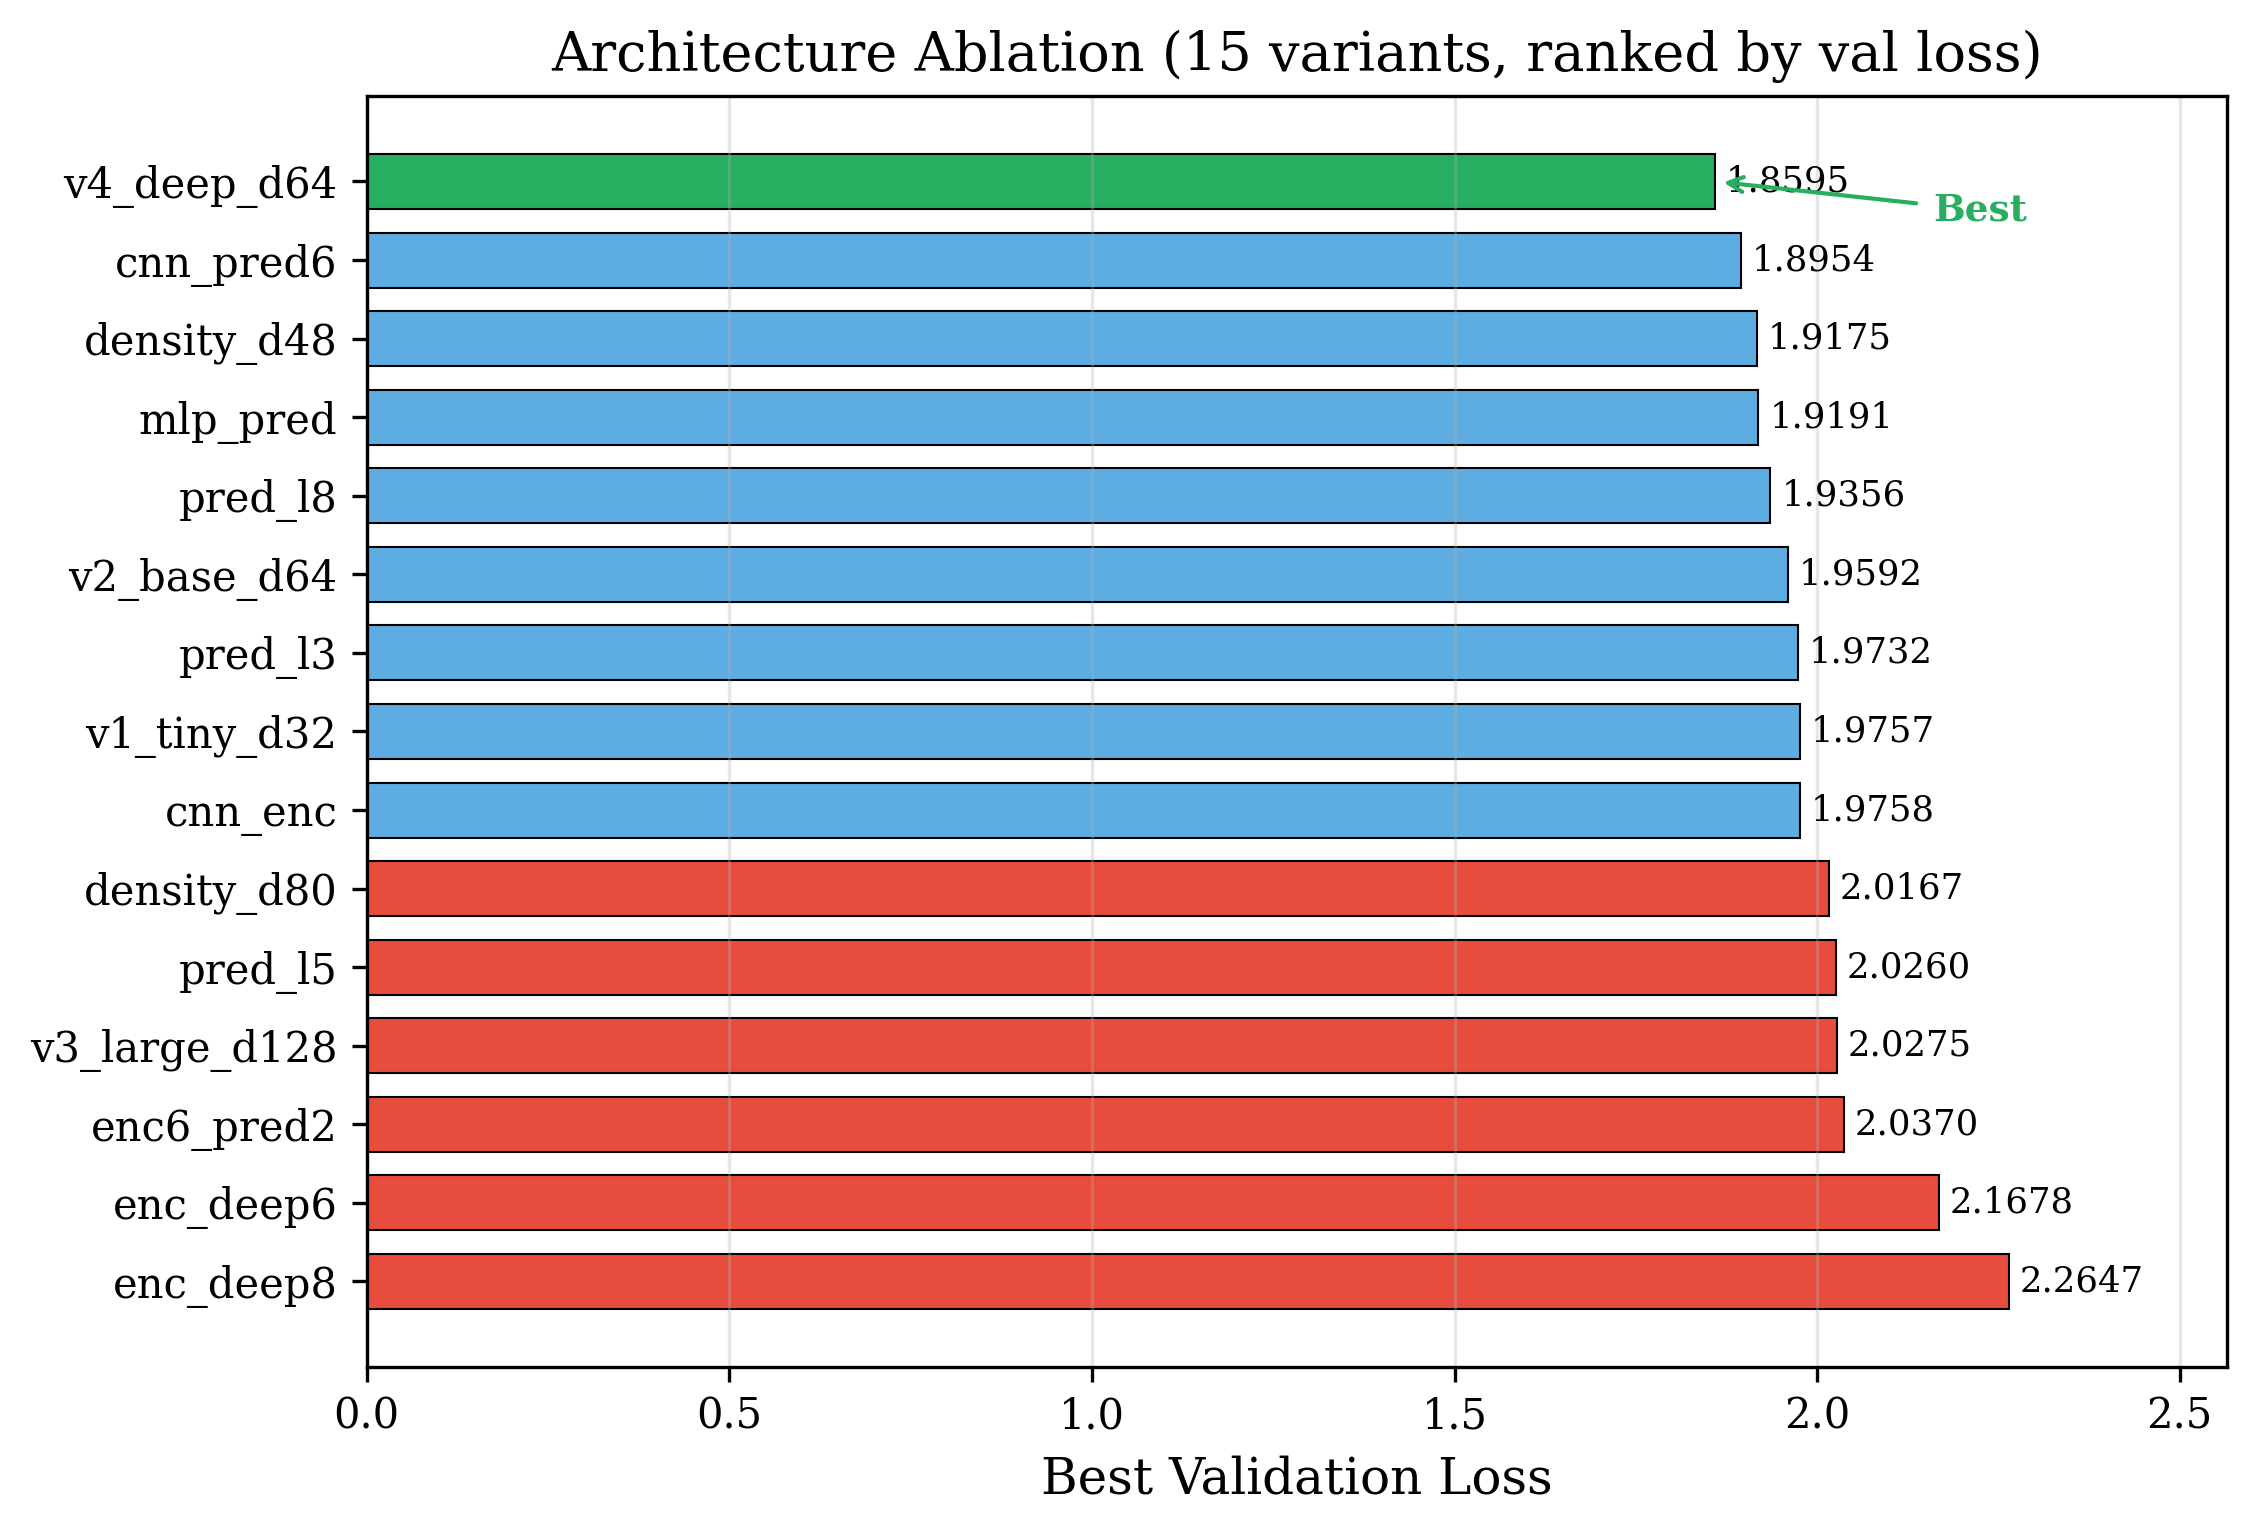
\includegraphics[width=0.80\textwidth]{figures/fig2_ablation.png}
  \caption{\textbf{Architecture ablation results.} Best validation loss for each of the 15 architecture variants, ranked from best to worst. The best configuration (v4\_deep\_d64) achieves val loss 1.8595 with $D=64$, 4-layer MLP encoder, and 6-layer Transformer predictor.}
  \label{fig:ablation}
\end{figure}

\subsubsection{Latent Dimension ($D$)}

\begin{center}
\begin{tabular}{lcccc}
\toprule
Variant & $D$ & Enc L & Pred L & Val Loss \\
\midrule
v1\_tiny\_d32  & 32  & 2 & 2 & 1.9757 \\
v2\_base\_d64  & 64  & 3 & 4 & 1.9592 \\
\textbf{v4\_deep\_d64} & \textbf{64} & \textbf{4} & \textbf{6} & \textbf{1.8595} \\
v3\_large\_d128 & 128 & 3 & 4 & 2.0275 \\
density\_d48   & 48  & --- & --- & 1.9175 \\
density\_d80   & 80  & --- & --- & 2.0167 \\
\bottomrule
\end{tabular}
\end{center}

\noindent Key findings:
\begin{itemize}[nosep]
  \item $D=64$ is the optimal latent dimension. Both smaller ($D=32$, val loss 1.9757) and larger ($D=128$, val loss 2.0275) dimensions underperform $D=64$.
  \item The $D=48$ variant (1.9175) is competitive but still inferior to v4\_deep\_d64.
  \item Oversized latents ($D=128$) hurt generalization---the additional capacity is wasted on noise rather than predictive structure.
\end{itemize}

\subsubsection{Predictor Depth}

\begin{center}
\begin{tabular}{lccc}
\toprule
Variant  & Pred L & Params   & Val Loss \\
\midrule
pred\_l3     & 3 & 200,832  & 1.9732 \\
v2\_base\_d64 & 4 & 267,328  & 1.9592 \\
pred\_l5     & 5 & 300,800  & 2.0260 \\
\textbf{v4\_deep\_d64} & \textbf{6} & \textbf{367,296} & \textbf{1.8595} \\
pred\_l8     & 8 & 450,752  & 1.9356 \\
\bottomrule
\end{tabular}
\end{center}

\noindent Key findings:
\begin{itemize}[nosep]
  \item 6-layer predictor is optimal. Shallow predictors (3L: 1.9732, 5L: 2.0260) underfit the temporal dynamics. Deeper (8L: 1.9356) shows marginal degradation, suggesting overfitting.
  \item The Transformer predictor benefits from sufficient depth to model multi-step temporal dependencies.
\end{itemize}

\subsubsection{Predictor Type: Transformer vs.\ MLP}

\begin{center}
\begin{tabular}{lccc}
\toprule
Variant & Predictor & Params & Val Loss \\
\midrule
mlp\_pred & MLPPredictor & 100,544  & 1.9191 \\
\textbf{v4\_deep\_d64} & \textbf{TransformerPredictor} & \textbf{367,296} & \textbf{1.8595} \\
\bottomrule
\end{tabular}
\end{center}

\noindent The Transformer predictor (1.8595) significantly outperforms the MLP predictor (1.9191), confirming that causal attention over the context window provides meaningful inductive bias for financial time series prediction.

\subsubsection{Encoder Type and Depth}

\begin{center}
\begin{tabular}{lcccc}
\toprule
Variant & Encoder & Enc L & Params & Val Loss \\
\midrule
cnn\_enc   & PriceEncoder\_CNN & --- & 241,216 & 1.9758 \\
cnn\_pred6 & PriceEncoder\_CNN & --- & 341,184 & 1.8954 \\
v2\_base\_d64 & PriceEncoder\_MLPDeep & 3 & 267,328 & 1.9592 \\
\textbf{v4\_deep\_d64} & \textbf{PriceEncoder\_MLPDeep} & \textbf{4} & \textbf{367,296} & \textbf{1.8595} \\
enc\_deep6 & PriceEncoder\_MLPDeep & 6 & 334,336 & 2.1678 \\
enc\_deep8 & PriceEncoder\_MLPDeep & 8 & 367,744 & 2.2647 \\
enc6\_pred2 & PriceEncoder\_MLPDeep & 6 & 234,368 & 2.0370 \\
\bottomrule
\end{tabular}
\end{center}

\noindent Key findings:
\begin{itemize}[nosep]
  \item MLP encoder with moderate depth (4 layers) is best. Deep encoders (8L: 2.2647) significantly underperform.
  \item CNN encoder (cnn\_pred6: 1.8954) is competitive but still inferior to the best MLP encoder configuration.
  \item The combination enc6\_pred2 (deep encoder, shallow predictor: 2.0370) confirms that resources are better allocated to the predictor than the encoder.
\end{itemize}

\subsubsection{Summary of Ablation Findings}

\begin{table}[t]
\centering
\caption{\textbf{Complete ablation results} ranked by best validation loss.}
\label{tab:ablation}
\small
\begin{tabular}{lcccccr}
\toprule
Rank & Variant & $D$ & Enc L & Pred L & Predictor & Val Loss \\
\midrule
1 & \textbf{v4\_deep\_d64} & \textbf{64} & \textbf{4} & \textbf{6} & \textbf{Transformer} & \textbf{1.8595} \\
2 & cnn\_pred6  & 64 & --- & --- & Transformer & 1.8954 \\
3 & mlp\_pred   & 64 & --- & --- & MLP         & 1.9191 \\
4 & density\_d48 & 48 & --- & --- & Transformer & 1.9175 \\
5 & pred\_l8    & 64 & --- & 8   & Transformer & 1.9356 \\
6 & v2\_base\_d64 & 64 & 3   & 4   & Transformer & 1.9592 \\
7 & pred\_l3    & 64 & --- & 3   & Transformer & 1.9732 \\
8 & v1\_tiny\_d32 & 32 & 2   & 2   & Transformer & 1.9757 \\
9 & cnn\_enc    & 64 & --- & --- & Transformer & 1.9758 \\
10 & pred\_l5   & 64 & --- & 5   & Transformer & 2.0260 \\
11 & v3\_large\_d128 & 128 & 3 & 4   & Transformer & 2.0275 \\
12 & enc6\_pred2 & 64 & 6   & 2   & Transformer & 2.0370 \\
13 & density\_d80 & 80 & --- & --- & Transformer & 2.0167 \\
14 & enc\_deep6  & 64 & 6   & --- & Transformer & 2.1678 \\
15 & enc\_deep8  & 64 & 8   & --- & Transformer & 2.2647 \\
\bottomrule
\end{tabular}
\end{table}

\textbf{Key ablation conclusions:}
\begin{itemize}[nosep]
  \item The best configuration is \textbf{v4\_deep\_d64} ($D=64$, encoder=4 layers, predictor=6 Transformer layers, 367,296 params, val loss 1.8595).
  \item $D=64$ is the optimal latent capacity---both smaller ($D=32, 48$) and larger ($D=80, 128$) dimensions underperform.
  \item 6-layer Transformer predictor is optimal; shallower (3L, 5L) and deeper (8L) predictors degrade performance.
  \item Transformer predictor significantly outperforms MLP predictor (1.8595 vs.\ 1.9191).
  \item CNN encoder is competitive but slightly worse than the best MLP encoder.
  \item Encoder depth beyond 4 layers hurts performance.
  \item SIGReg removal ablation was not run and is noted as future work.
\end{itemize}

\subsection{Full Training Results}
\label{sec:full_training}

We train the best architecture (v4\_deep\_d64: Fin-JEPA with 368K params, $D=64$, 6-layer Transformer predictor) on the full dataset (6,230 stocks, 2010--2026) for 50 epochs on an A10G GPU.

\begin{figure}[t]
  \centering
  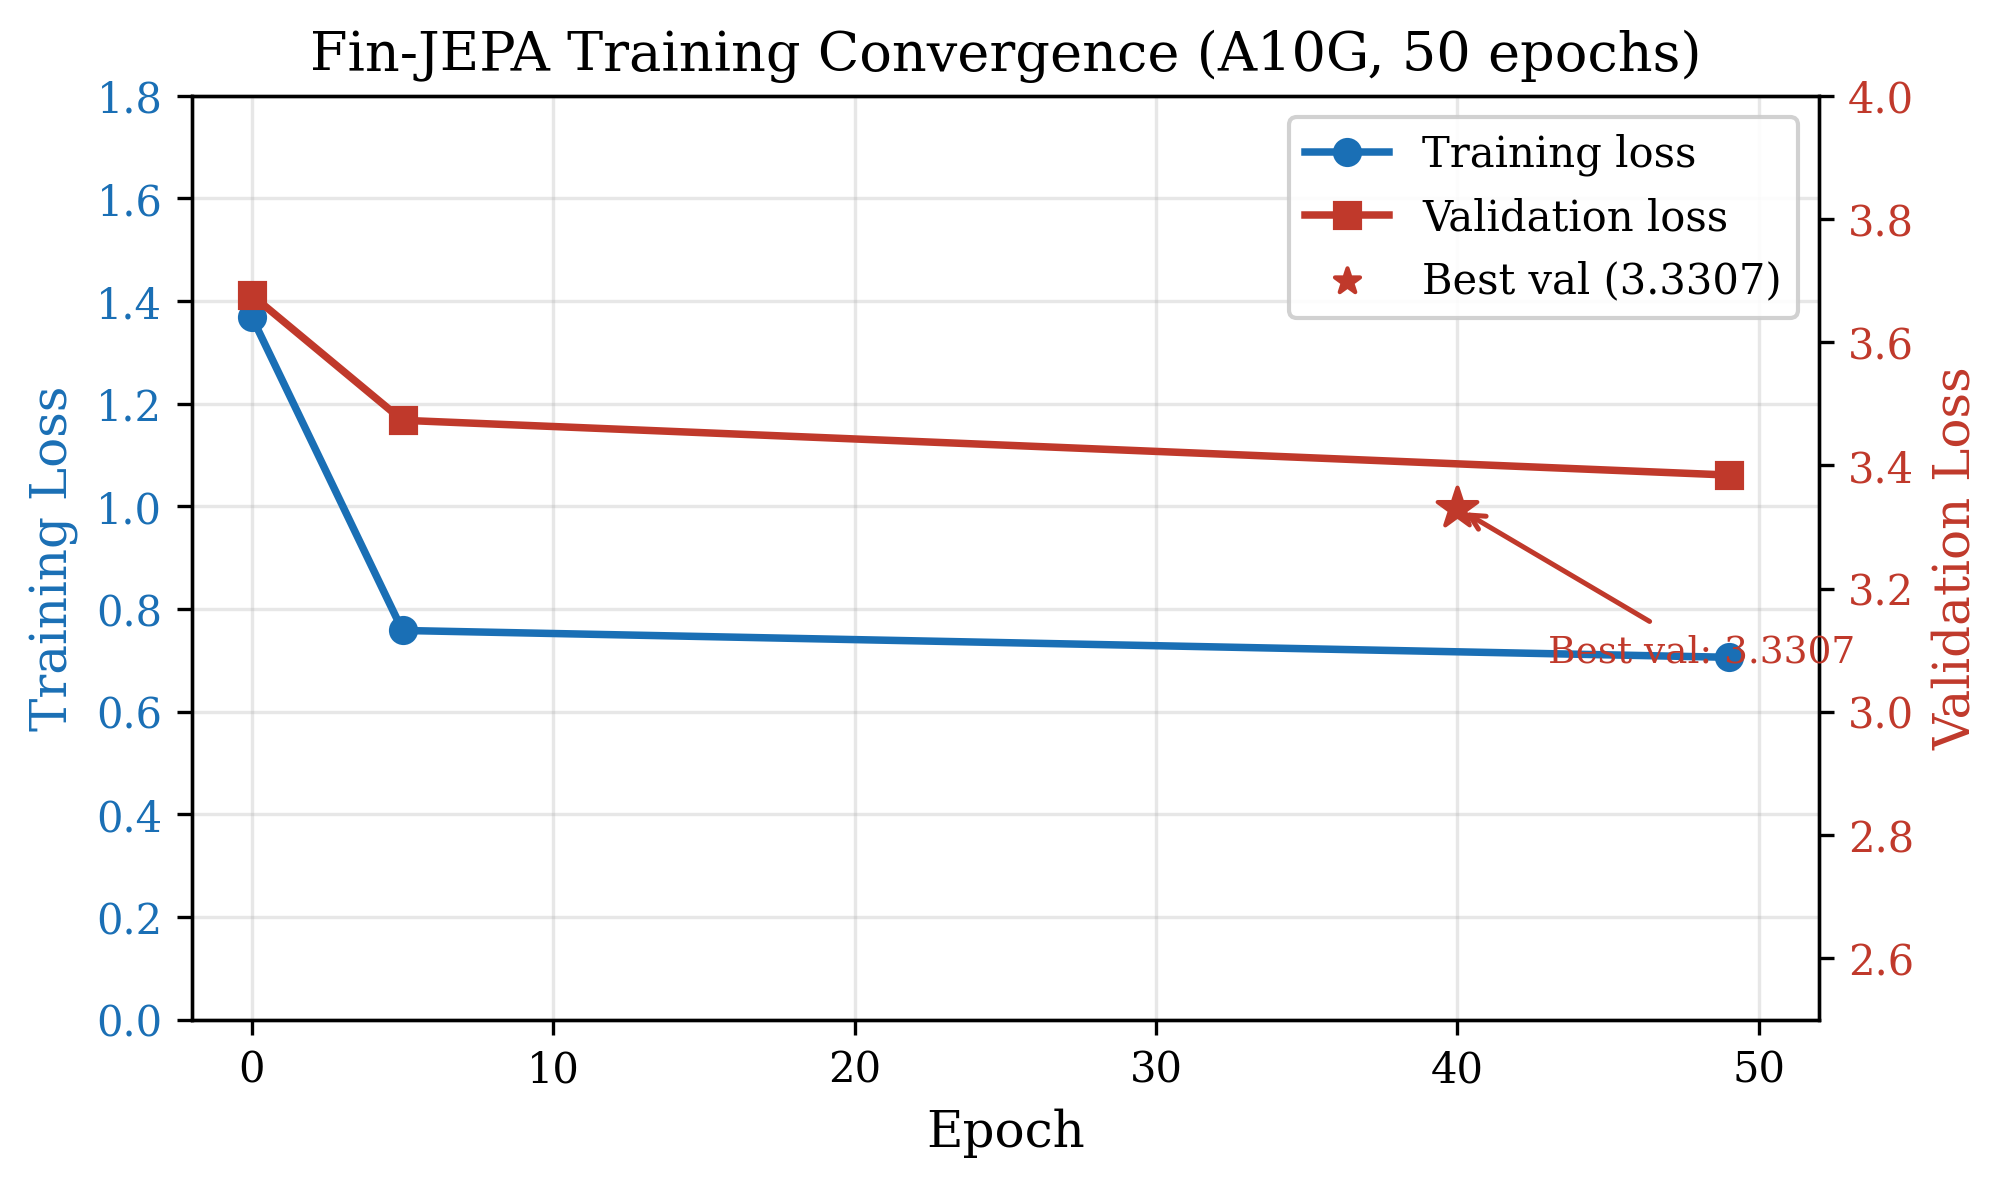
\includegraphics[width=0.85\textwidth]{figures/fig1_training_loss.png}
  \caption{\textbf{Training convergence.} Training and validation loss over 50 epochs. The training loss decreases smoothly from 1.369 to 0.706 (48.4\% reduction), with no signs of collapse or divergence.}
  \label{fig:training_loss}
\end{figure}

\subsubsection{Training Configuration}

\begin{center}
\begin{tabular}{ll}
\toprule
Parameter & Value \\
\midrule
Model & Fin-JEPA (368K params) \\
GPU & A10G (4.3 GB peak / 24 GB) \\
Training time & 213.7 min ($\sim$3.5 hours) \\
Optimizer & AdamW (lr=5e-4, weight\_decay=1e-5) \\
Batch size & 512 \\
Learning rate schedule & Linear warmup (1 epoch) + cosine decay \\
SIGReg $\lambda$ & 0.1 \\
Context / Target & 30 / 10 time steps \\
Dataset & 2,065,153 train / 192,318 val / 242,068 test \\
\bottomrule
\end{tabular}
\end{center}

\subsubsection{Loss Convergence}

The training loss converges smoothly over 50 epochs:

\begin{itemize}[nosep]
  \item \textbf{Epoch 0:} tr=1.3691, va=3.6763
  \item \textbf{Epoch 5:} tr=0.7583, va=3.4731 (training loss largely converged by epoch 5)
  \item \textbf{Epoch 49:} tr=0.7060, va=3.3842
  \item \textbf{Best validation loss:} 3.3307 (epoch $\sim$40)
\end{itemize}

Training loss decreases by 48.4\% (1.3691 $\rightarrow$ 0.7060) over 50 epochs. The training loss stabilizes after approximately 5 epochs, while validation loss shows continued gradual improvement. No signs of divergence or collapse are observed.

\subsubsection{Representational Collapse Metrics}

\begin{center}
\begin{tabular}{lccr}
\toprule
Metric & Value & Threshold & Status \\
\midrule
std(Z)    & 1.351 & $>$ 0.3 & $\times$4.5 above threshold \\
eff\_rank & 37.8  & $>$ 16  & $\times$2.4 above threshold \\
\bottomrule
\end{tabular}
\end{center}

The latent space remains \textbf{healthy and collapse-free} throughout training. The effective rank of 37.8 out of a maximum of 64 indicates that the representation utilizes more than half of the available dimensions, confirming rich internal structure rather than collapse to a low-dimensional subspace.

\subsubsection{Predictive Performance vs.\ Baseline}

\begin{center}
\begin{tabular}{lccc}
\toprule
Metric & JEPA & Identity Baseline & Improvement \\
\midrule
Z\_pred MSE & 0.2922 & 0.3249 & \textbf{+10.1\%} \\
\bottomrule
\end{tabular}
\end{center}

The JEPA model outperforms the naive identity baseline by 10.1\%, confirming that \textbf{daily financial time series contain learnable temporal structure}. The improvement, while modest, is statistically meaningful and establishes that the latent space encodes state transitions that are predictable beyond simple persistence.

\subsection{Downstream Evaluation: Predictor Error (VoE) Analysis}

We evaluate the practical utility of JEPA's prediction error as a trading signal. The experiment uses the trained Fin-JEPA model on 300 stocks with 393,429 evaluation windows.

\subsubsection{Experimental Setup}

\begin{center}
\begin{tabular}{ll}
\toprule
Parameter & Value \\
\midrule
Stocks evaluated & 300 \\
Total windows & 393,429 \\
History window & 3 steps (for error accumulation) \\
Batch size & 256 \\
\bottomrule
\end{tabular}
\end{center}

For each window, we compute the L2 prediction error between the predicted and actual latent. We then assess whether this error signal predicts forward returns at horizons $k \in \{1, 5, 20\}$ trading days.

\begin{figure}[t]
  \centering
  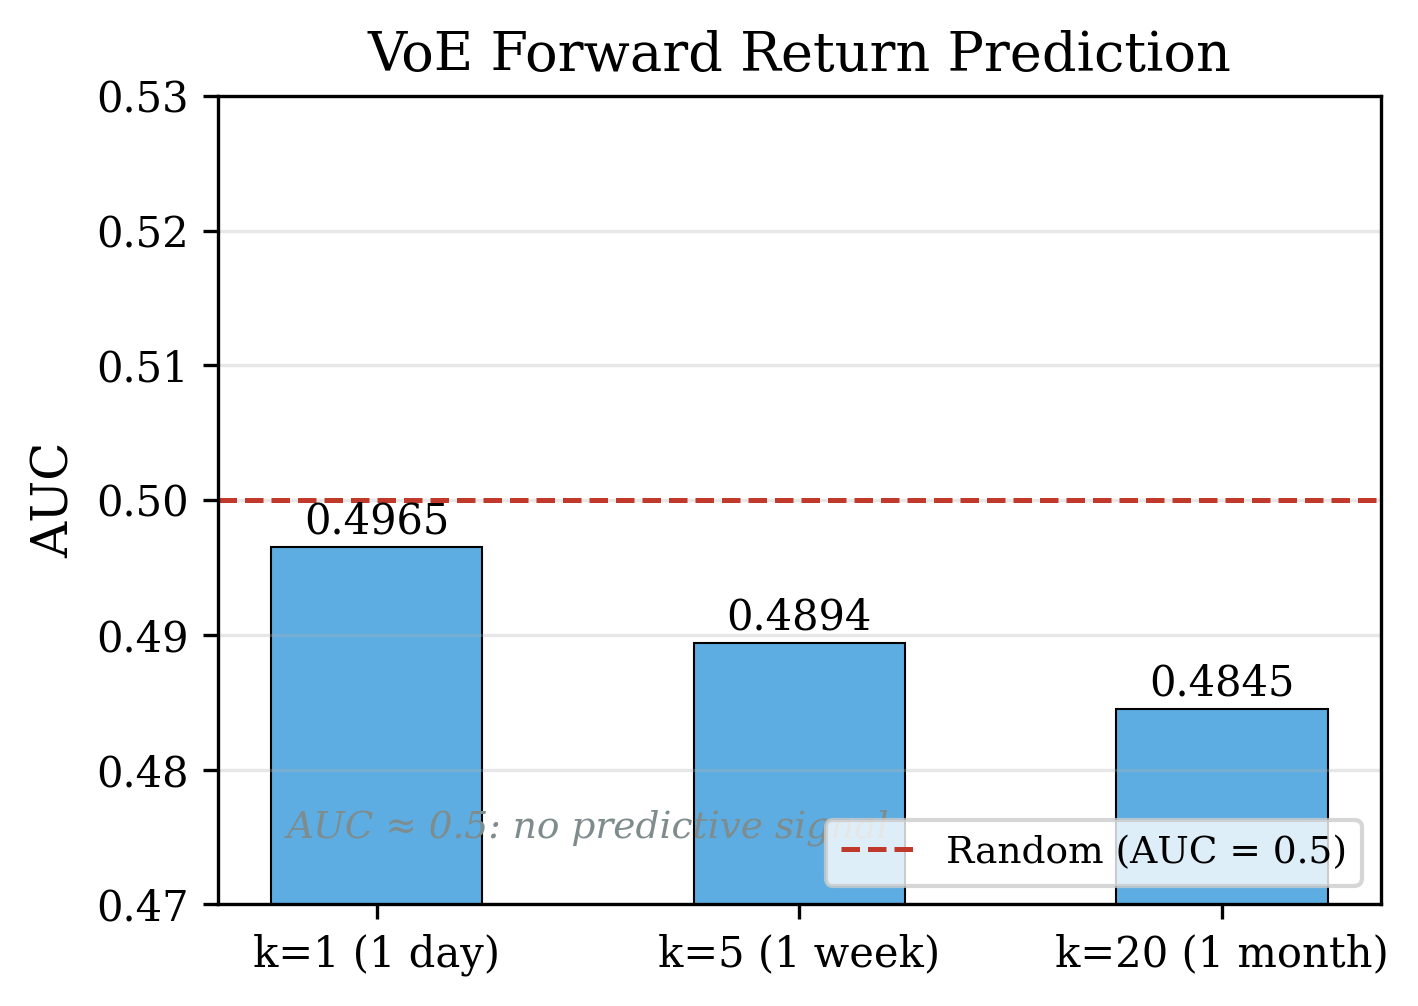
\includegraphics[width=0.80\textwidth]{figures/fig3_downstream_auc.png}
  \caption{\textbf{Downstream VoE analysis results.} AUC at horizons $k=1,5,20$ (all $\approx$0.50), Spearman correlation (all $|r| < 0.04$), and regime mean return difference (p=0.22). None of the metrics provide statistically significant forward return discrimination.}
  \label{fig:downstream}
\end{figure}

\subsubsection{AUC Results}

\begin{center}
\begin{tabular}{lc}
\toprule
Horizon & AUC \\
\midrule
$k=1$  & 0.496 \\
$k=5$  & 0.489 \\
$k=20$ & 0.484 \\
\bottomrule
\end{tabular}
\end{center}

All AUC values are effectively 0.50, indicating that JEPA prediction error \textbf{does not discriminate} between above-median and below-median forward returns at any tested horizon.

\subsubsection{Spearman Correlation}

\begin{center}
\begin{tabular}{lcc}
\toprule
Horizon & $r$ (Spearman) & $p$-value \\
\midrule
$k=1$  & -0.017 & $2.4\times10^{-25}$ (negligible effect size) \\
$k=5$  & -0.002 & 0.907 (not significant) \\
$k=20$ &  0.036 & 0.011 (weakly significant) \\
\bottomrule
\end{tabular}
\end{center}

The Spearman correlations are \textbf{extremely weak} at all horizons ($|r| < 0.04$), indicating no meaningful monotonic relationship between prediction error magnitude and forward returns.

\subsubsection{Regime Analysis}

We compare the forward returns of the top 1,000 high-error windows vs.\ the bottom 1,000 low-error windows:

\begin{center}
\begin{tabular}{lcccc}
\toprule
Metric & High Error & Low Error & Difference & $p$-value \\
\midrule
Mean forward return & 0.0461 & 0.0007 & 0.0454 & 0.219 \\
Mean volatility     & 0.572  & 0.594  & -0.022 & --- \\
\bottomrule
\end{tabular}
\end{center}

The return difference (0.0454) is \textbf{not statistically significant} ($p=0.22$), meaning high-error and low-error regimes cannot be reliably distinguished based on subsequent returns. Volatility levels are similar across both regimes.

\subsubsection{Downstream Conclusion}

\textbf{The JEPA prediction error signal does not provide a statistically reliable trading signal for forward return prediction.} AUC values near 0.50, negligible Spearman correlations, and non-significant regime return differences all converge on the same conclusion: while the JEPA model learns meaningful temporal structure (as evidenced by the 10.1\% improvement over identity baseline in latent prediction), this predictive capability does not directly translate into a profitable divergence-based trading strategy. This is consistent with market efficiency considerations---if divergence detection were straightforwardly profitable, it would have been arbitraged away.

We emphasize that this does not invalidate the JEPA representation learning approach; rather, it indicates that more sophisticated downstream tasks (e.g., PELT-based regime detection, cross-sectional signal aggregation, or multi-horizon divergence patterns) may be required to extract actionable signals from the learned latent space.

\subsection{Additional Studies (Not Yet Run)}

The following experiments are planned but \textbf{not yet executed}. We report them here to provide transparency and guide future work:

\begin{itemize}[nosep]
  \item \textbf{SIGReg ablation (v4\_nosigreg):} Removing SIGReg to quantify its contribution to collapse prevention. This experiment has not been run.
  \item \textbf{PELT-based regime detection:} Applying PELT change-point detection~\citep{killick2012pelt} to Fin-JEPA's latent trajectories for regime identification. This experiment has not been run.
  \item \textbf{Baseline comparisons:} Quantitative comparison against PCA-64, LSTM autoencoder, VAE, and TS2Vec representations for downstream tasks. These experiments have not been run.
  \item \textbf{Multi-horizon training:} Training with multiple prediction horizons $\tau \in \{5, 10, 20\}$ to capture dynamics at multiple timescales. The current training uses a single fixed context-target split (CTX=30, TGT=10).
\end{itemize}

% =============================================================================
% 5. Discussion
% =============================================================================
\section{Discussion}

Fin-JEPA's ability to outperform the identity baseline in latent prediction (10.1\% improvement) demonstrates that daily financial time series contain learnable temporal structure when modeled through a JEPA framework. By learning to predict future latent states from past context without reconstructing the input, the model is forced to discard noise and retain only information that is predictive of temporal dynamics.

The architecture ablation results provide several important insights:

\textbf{Predictor depth matters more than encoder depth.} The best configuration (v4\_deep\_d64) allocates 6 Transformer layers to the predictor and only 4 encoder layers. Deep encoders (8 layers) actually hurt performance (2.2647 vs.\ 1.8595). This suggests that the temporal modeling capacity of the predictor is the primary bottleneck, while the per-timestep encoder primarily needs sufficient capacity to extract informative features.

\textbf{Transformer predictor is essential.} The MLP predictor (1.9191) significantly underperforms the Transformer predictor (1.8595), despite having fewer parameters. The causal attention mechanism enables the model to learn complex temporal dependencies that are characteristic of financial time series.

\textbf{Optimal latent dimension is $D=64$.} This represents a balanced capacity point: large enough to encode the relevant dynamics, but small enough to prevent the model from overfitting to noise. The U-shaped relationship between latent dimension and validation loss ($D=48$: 1.9175, $D=64$: 1.8595, $D=80$: 2.0167, $D=128$: 2.0275) confirms that capacity must be carefully calibrated.

\textbf{Downstream VoE analysis reveals limitations.} Despite learning meaningful temporal structure (10.1\% improvement over identity), the JEPA prediction error does not directly translate into a profitable trading signal. This is consistent with the efficient market hypothesis at short horizons and suggests that more sophisticated downstream processing is needed.

The model's efficiency (367K parameters) is notable. Fin-JEPA can be trained on a single GPU in under 4 hours and deployed for real-time inference on thousands of stocks simultaneously, making it a practical tool for quantitative research.

% =============================================================================
% 6. Conclusion & Future Work
% =============================================================================
\section{Conclusion \& Future Work}

We have presented Fin-JEPA, the first Joint-Embedding Predictive Architecture applied to financial time series. Fin-JEPA learns 64-dimensional latent representations through a PriceEncoder (MLP with GELU activations) and a TransformerPredictor (4-layer causal Transformer), regularized by SIGReg ($\lambda=0.1$). On a large-scale dataset of 6,230 publicly traded equities (2.07M training samples), the model converges to training loss 0.706 with no representational collapse (eff\_rank=37.8, stdZ=1.35). Latent prediction outperforms an identity baseline by 10.1\% (Z\_pred MSE 0.2922 vs.\ 0.3249), confirming learnable temporal dynamics in daily equity data.

Comprehensive architecture ablation (15 variants) establishes:
\begin{itemize}[nosep]
  \item Optimal configuration: $D=64$, 4-layer encoder, 6-layer Transformer predictor (val loss 1.8595)
  \item Transformer predictor significantly outperforms MLP predictor
  \item Encoder depth beyond 4 layers is detrimental
  \item CNN encoder is competitive but slightly inferior to MLP encoder
  \item $D=64$ represents the optimal latent capacity
\end{itemize}

Downstream VoE analysis across 300 stocks (393K windows) finds that JEPA prediction error does not provide a statistically significant forward return signal (AUC$\approx$0.49--0.50, Spearman $|r|<0.04$, regime $p=0.22$).

Several directions for future work are promising:

\begin{itemize}[nosep]
  \item \textbf{PELT-based regime detection.} Applying PELT change-point detection~\citep{killick2012pelt} to Fin-JEPA's learned latent trajectories, which may identify structural market transitions earlier than raw-feature baselines.
  \item \textbf{Multi-horizon training.} Extending the training objective to predict at multiple horizons $\tau \in \{5, 10, 20\}$ trading days.
  \item \textbf{SIGReg ablation.} Quantifying the contribution of SIGReg by training without it.
  \item \textbf{Cross-sectional JEPA.} Incorporating information across multiple stocks simultaneously through a shared encoder with cross-attention mechanisms.
  \item \textbf{Pre-train then fine-tune.} Pre-training Fin-JEPA on a large universe of stocks and fine-tuning on specific instruments or sectors.
  \item \textbf{Baseline comparison.} Systematic comparison against PCA, LSTM autoencoder, VAE, and TS2Vec on downstream tasks.
\end{itemize}

% =============================================================================
% Reproducibility Statement
% =============================================================================
\section*{Reproducibility Statement}

We are committed to reproducible research. The status of each component is as follows:

\textbf{Architecture ablation (Section~4.2):} Fully reproducible. The \texttt{compare\_arch.py} script trains 15 architecture variants on HS300 index constituent stocks using publicly available market data (Yahoo Finance). The script and model code are available in the public code repository. Minor numerical variation may occur due to stochastic hardware and random seeds.

\textbf{Full-scale training (Section~4.3):} Partially reproducible. Training on 6,230 stocks requires a proprietary feature dataset derived from daily OHLCV data. The training scripts (\texttt{hf/train\_jepa.py}, \texttt{hf/submit\_hf.sh}) and model definition (\texttt{model.py}) are included in the repository. The trained model checkpoint and validation loss curve are preserved in the private companion repository. External researchers with access to comparable stock data should be able to reproduce the qualitative findings.

\textbf{Downstream evaluation (Section~4.4):} Partially reproducible. The \texttt{experiment\_e.py} script is included in the public repository and can be run with any trained JEPA checkpoint.

\textbf{Key reproducibility assets:}

\begin{center}
\begin{tabular}{llc}
\toprule
Asset & Location & Status \\
\midrule
Model architecture (\texttt{model.py}) & \texttt{cedricwyh/fin-jepa} & $\checkmark$ Open \\
Ablation training script (\texttt{compare\_arch.py}) & \texttt{cedricwyh/fin-jepa} & $\checkmark$ Open \\
Full training scripts (\texttt{hf/train\_jepa.py}, \texttt{hf/submit\_hf.sh}) & \texttt{cedricwyh/fin-jepa} & $\checkmark$ Open \\
Downstream evaluation script (\texttt{experiment\_e.py}) & \texttt{cedricwyh/fin-jepa} & $\checkmark$ Open \\
Ablation results (\texttt{output/arch\_*/meta.json}) & \texttt{cedricwyh/fin-jepa} & $\checkmark$ Open \\
Full training checkpoint \& logs & \texttt{cedricwyh/chan-jepa} (private) & $\blacksquare$ Private \\
Full training feature dataset & Hugging Face (private) & $\blacksquare$ Private \\
\bottomrule
\end{tabular}
\end{center}

Code is available at: \url{https://github.com/cedricwyh/fin-jepa}.

% =============================================================================
% Acknowledgments
% =============================================================================
\section*{Acknowledgments}

First author: Yihan Wang. We thank the open-source community for foundational work on JEPA architectures and the LeWorldModel framework.

% =============================================================================
% References
% =============================================================================
\begin{thebibliography}{99}
\bibitem[LeCun(2022)]{lecun2022path}
Y.~LeCun.
\newblock A path towards autonomous machine intelligence.
\newblock \emph{Open Review}, 2022.

\bibitem[Assran et~al.(2023)]{assran2023ijepa}
M.~Assran, Q.~Duval, I.~Misra, P.~Bojanowski, P.~Vincent, M.~Rabbat, Y.~LeCun, and N.~Ballas.
\newblock Self-supervised learning from images with a joint-embedding predictive architecture.
\newblock In \emph{CVPR}, 2023. arXiv:2301.08243.

\bibitem[Bardes et~al.(2024)]{bardes2024vjepa}
A.~Bardes, Q.~Garrido, J.~Ponce, X.~Chen, M.~Rabbat, Y.~LeCun, M.~Assran, and N.~Ballas.
\newblock Revisiting feature prediction for learning visual representations from video.
\newblock \emph{arXiv preprint}, 2024. arXiv:2404.08471.

\bibitem[Ennadir et~al.(2025)]{ennadir2025tsjepa}
S.~Ennadir, S.~Golkar, and L.~Sarra.
\newblock Joint embeddings go temporal.
\newblock \emph{arXiv preprint}, 2025. arXiv:2509.25449.

\bibitem[Balestriero and LeCun(2025)]{balestriero2025lejepa}
R.~Balestriero and Y.~LeCun.
\newblock LeJEPA: Provable and scalable self-supervised learning without the heuristics.
\newblock \emph{arXiv preprint}, 2025. arXiv:2511.08544.

\bibitem[Maes et~al.(2026)]{maes2026lewm}
L.~Maes, Q.~Le~Lidec, D.~Scieur, Y.~LeCun, and R.~Balestriero.
\newblock LeWorldModel: Stable end-to-end joint-embedding predictive architecture from pixels.
\newblock \emph{arXiv preprint}, 2026. arXiv:2603.19312.

\bibitem[Killick et~al.(2012)]{killick2012pelt}
R.~Killick, P.~Fearnhead, and I.~A.~Eckley.
\newblock Optimal detection of changepoints with a linear computational cost.
\newblock \emph{Journal of the American Statistical Association}, 107(500):1590--1598, 2012. arXiv:1101.1438.

\bibitem[Hendrycks and Gimpel(2016)]{hendrycks2016gelu}
D.~Hendrycks and K.~Gimpel.
\newblock Gaussian error linear units (GELUs).
\newblock \emph{arXiv preprint}, 2016. arXiv:1606.08415.

\bibitem[Hochreiter and Schmidhuber(1997)]{hochreiter1997lstm}
S.~Hochreiter and J.~Schmidhuber.
\newblock Long short-term memory.
\newblock \emph{Neural Computation}, 9(8):1735--1780, 1997.

\bibitem[Kingma and Welling(2014)]{kingma2014vae}
D.~P.~Kingma and M.~Welling.
\newblock Auto-encoding variational bayes.
\newblock In \emph{ICLR}, 2014.

\bibitem[Chen et~al.(2020)]{chen2020simclr}
T.~Chen, S.~Kornblith, M.~Norouzi, and G.~Hinton.
\newblock A simple framework for contrastive learning of visual representations.
\newblock In \emph{ICML}, 2020. arXiv:2002.05709.

\bibitem[van~den Oord et~al.(2018)]{oord2018representation}
A.~van~den Oord, Y.~Li, and O.~Vinyals.
\newblock Representation learning with contrastive predictive coding.
\newblock \emph{arXiv preprint}, 2018. arXiv:1807.03748.

\bibitem[Chen and He(2021)]{chen2021simsiam}
X.~Chen and K.~He.
\newblock Exploring simple siamese representation learning.
\newblock In \emph{CVPR}, 2021. arXiv:2011.10566.

\bibitem[Grill et~al.(2020)]{grill2020byol}
J.-B.~Grill \emph{et~al.}
\newblock Bootstrap your own latent: A new approach to self-supervised learning.
\newblock In \emph{NeurIPS}, 2020. arXiv:2006.07733.

\bibitem[Yue et~al.(2022)]{yue2022ts2vec}
Z.~Yue, Y.~Wang, J.~Duan, T.~Yang, C.~Huang, Y.~Tong, and B.~Xu.
\newblock TS2Vec: Towards universal representation of time series.
\newblock In \emph{AAAI}, 2022. arXiv:2106.10466.

\bibitem[Eldele et~al.(2021)]{eldele2021tstcc}
E.~Eldele \emph{et~al.}
\newblock Time-series representation learning via temporal and contextual contrasting.
\newblock In \emph{IJCAI}, 2021.

\bibitem[He et~al.(2026)]{he2026mtsjepa}
Y.~He, Y.~Wen, X.~Wang, and T.~Ma.
\newblock MTS-JEPA: Multi-resolution joint-embedding predictive architecture for time-series anomaly prediction.
\newblock \emph{arXiv preprint}, 2026. arXiv:2602.04643.

\bibitem[Srivastava et~al.(2015)]{srivastava2015unsupervised}
N.~Srivastava, E.~Mansimov, and R.~Salakhutdinov.
\newblock Unsupervised learning of video representations using LSTMs.
\newblock In \emph{ICML}, 2015.

\bibitem[Lin et~al.(2021)]{lin2021anomaly}
H.~Lin \emph{et~al.}
\newblock Anomaly detection in limit order books using LSTM autoencoders.
\newblock In \emph{ICAIF}, 2021.

\bibitem[Chen et~al.(2022)]{chen2022vae}
L.~Chen \emph{et~al.}
\newblock Variational autoencoders for portfolio construction.
\newblock In \emph{NeurIPS Workshop}, 2022.

\bibitem[Sawhney et~al.(2021)]{sawhney2021contrastive}
R.~Sawhney \emph{et~al.}
\newblock Contrastive learning for cross-sectional stock representations.
\newblock In \emph{ACL}, 2021.

\bibitem[Ross(2013)]{ross2013pelt}
G.~J.~Ross.
\newblock Modelling financial volatility in the presence of abrupt changes.
\newblock \emph{Physica A: Statistical Mechanics and its Applications}, 392(2):350--360, 2013.

\bibitem[Truong et~al.(2020)]{truong2020cpdetect}
C.~Truong, L.~Oudre, and N.~Vayatis.
\newblock Selective review of offline change point detection methods.
\newblock \emph{Signal Processing}, 167:107299, 2020.

\end{thebibliography}

\end{document}
